Um escoamento monofásico, permanente e plenamente desenvolvido
de um fluido newtoniano e incompressível 
entre placas horizontais paralelas e imóveis é 
mantido em virtude de um gradiente de pressão 
$\partial p/\partial x$ imposto conforme mencionado por Pontes e Mangiavacchi (2016) \cite{pontes2016}.
Este escoamento é conhecido como \textit{Escoamento de Poiseuille}.
A \ref{poiseuille} apresenta esquematicamente este escoamento e
o perfil do campo de velocidade esperado.

A monophase, steady and fully developed flow of a Newtonian 
and incompressible fluid between parallel and fixed horizontal 
plates is maintained due to a pressure gradient 
$\partial p/ \partial x$ imposed as mentioned by Pontes 
and Mangiavacchi (2016) \cite{pontes2016}. 
This flow is known as \textit{Poiseuille flow}. 
\ref{poiseuille} presents schematically this flow and 
the expected velocity field.

\begin{figure}[H]
\begin{center}
\begin{tikzpicture}[scale=1.3]
 \draw [pattern=north east lines] (0,0) -- (0,-0.1) -- (5,-0.1) -- (5,0) -- cycle;
 \draw [pattern=north east lines] (0,1) -- (0,1.1) -- (5,1.1) -- (5,1) -- cycle;

 \draw [->,thick] (-2,-0.1)--(-2,1.5) node[left] {$y$};
 \draw [->,thick] (-2.1,0)--(-0.5,0) node[below] {$x$};
 
 \draw [dotted] (2.5,0.0) to (2.5,1.0);
 \draw  (2.5,0.0) to [bend right=100] (2.5,1.0);
 
 \draw [->,thick] (2.5,0.9) to (2.7,0.9);
 \draw [->,thick] (2.5,0.7) to (2.78,0.7);
 \draw [->,thick] (2.5,0.5) to (2.8,0.5);
 \draw [->,thick] (2.5,0.3) to (2.78,0.3);
 \draw [->,thick] (2.5,0.1) to (2.7,0.1);
\end{tikzpicture}
\end{center}
\caption{Poiseuille Flow}
\label{poiseuille}
\end{figure}

\noindent
The velocity profile equation is shown below:

\begin{equation}
 u = \frac{4 u_{max}}{L^2} y \big[ L - y \big]
\end{equation}

\medskip
\noindent
where $u_{max}$ is maximum velocity and its value is 
$u_{max} = 1.5$, $L$ is non-dimensional length 
between the plates and its value is 
$L = 1$
and $y$ is the vertical coordinates and it varies 
between $y = \big[ 0,1 \big]$.
The domain was discretized using a linear triangular mesh
with 3835 nodes and 7299 elements.

\medskip
\noindent
The boundary conditions used was:

\begin{itemize}
     \item \textit{inflow}:
      the normal velocity component is null $v=0$, 
      while the tangencial velocity component is set analytical profile
      $u = u_{analytical}$.

     \item \textit{noslip}: this condition is used in the plates,
      where all velocity components is null $u=0$ and $v=0$.
      The streamfunction field is ,  
$\psi=1$ in top plate and
$\psi=0$ in bottom plate.

     \item \textit{condição de saída}: O valor da função de corrente é especificado $\psi=y$. As derivadas das
     componentes tangencial e normal da velocidade possuem o 
     valor nulo, isto é,
      $\partial u/\partial n = 0$ e
      $\partial v/\partial n = 0$ respectivamente.
\end{itemize}


\medskip
A \ref{velocidade poiseuille} apresenta a evolução 
do perfil de velocidade no tempo quando o $Re=100$, além do comparativo
entre a solução numérica e a solução analítica no estado permanente do
problema proposto. 


\begin{figure}[H]
     \centering
     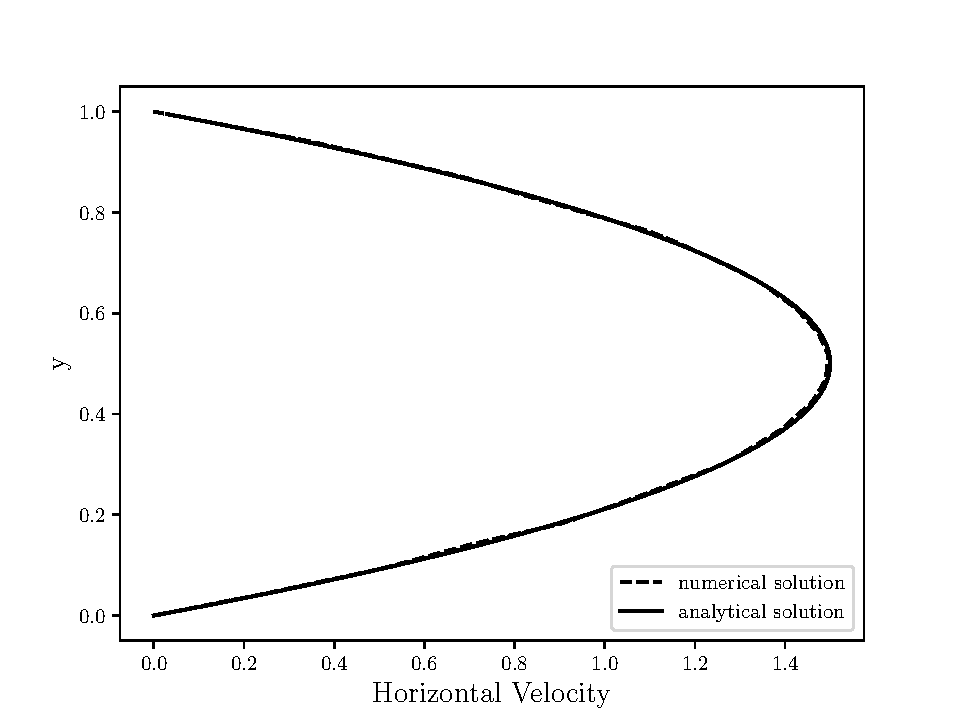
\includegraphics[scale=1]{./02_chaps/cap_validation/figure/poiseuille_velocity.pdf}\\
     \medskip
     \caption{Evolução do perfil de velocidade no tempo e
     a comparação da solução numérica no estado permanente com a solução analítica para o Escoamento de Poiseuille.}
     \label{velocidade poiseuille}
\end{figure}

\newpage
A \ref{erro relativo poiseuille tabela} apresenta o erro relativo
entre a solução numérica e a solução analítica para diversas malhas
não estruturadas, variando entre 100 a 25600 elementos triangulares lineares.
Para a malha com 7299 elementos como no caso deste teste, o erro relativo estimado para o campo de
velocidade está entre as faixas 0,49\% e 0,13\%. 

\vspace{0.5cm}
\begin{table}[H]
\centering
\begin{tabular}{ccc}
\toprule
\textbf{N. Elementos} & \textbf{Erro} (\%) \\
\midrule
100 & 25,00 \\
400 & 7,27 \\
1600 & 1,94 \\
6400 & 0,49 \\
25600 & 0,13 \\
\bottomrule
\end{tabular}
\caption{Erro relativo da solução numérica para diferentes malhas não estruturadas}
\label{erro relativo poiseuille tabela}
\end{table}

\noindent
\medskip
O erro relativo foi estimado como:

\begin{equation}
 \mathit{Erro} = \sqrt{\frac{\sum{(v_{n} - v_{a})^{2} }}{\sum |v_{a}|^{2} }}
\end{equation}

\noindent
onde $v_{n}$ é o campo da velocidade numérica e $v_{a}$ é o campo
da velocidade analítica. 



\newpage
A \ref{ordem de convergencia poiseuille} apresenta o erro
relativo da solução numérica com as curvas de convergência de primeira e segunda ordem em uma
escala logaritmica. Como pode ser observado, o erro da solução numérica para diferentes números
de elementos triangulares lineares possui a forma de convergência de primeira ordem.
Dessa forma, ao aumentar o número de elementos, o erro relativo da solução numérica
regride linearmente.


\begin{figure}[H]
     \centering
     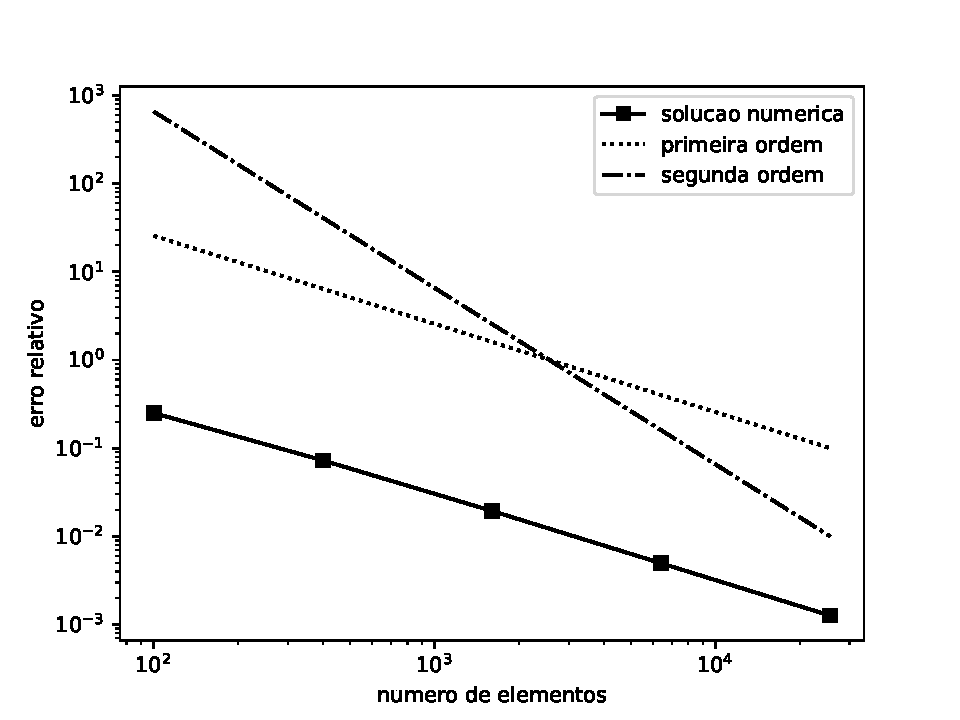
\includegraphics[scale=1]{./02_chaps/cap_validation/figure/poiseuille_error.pdf}\\
     \medskip
     \caption{Ordem de convergência em escala logaritmica. É estimado que o erro relativo
              da solução numérica possui convergência de primeira ordem.}
     \label{ordem de convergencia poiseuille}
\end{figure}


\newpage
